\graphicspath{{4sets/asy/}}
\section{Sets and Functions}\label{chap:sets}


Sets are the fundamental building blocks of mathematics, providing the language necessary for describing mathematical objects and for grouping objects together according to shared characteristics. Understanding how to read and effectively employ set notation is our primary focus. The mathematical discipline of \emph{set theory} is, however, far more ambitious than this. Set theorists define all basic mathematical objects---\emph{numbers, addition, functions,} etc.---purely in terms of sets, an impractical approach for most working mathematicians, most of the time.\footnote{Within \emph{axiomatic set theory} it can take over 100 pages to justify writing $1+1=2$. The difficulty is that rigorous definitions---using sets---are first required of the notions \emph{one, two, equals} and \emph{add}\ldots} We will only scratch the surface of this. Indeed long before one can accept that such an approach has its place in mathematics, a significant level of familiarity with sets and their basic operations is necessary.


\subsection{Set Notation and Subsets}\label{sec:subset}

Without any attempt to define the meaning of \emph{object,} we start with a naïve definition.

\begin{defn}[lower separated=false, sidebyside, sidebyside align=top seam, sidebyside gap=0pt, righthand width=0.3\linewidth]{}{}
	A \emph{set} is a collection of objects, its \emph{elements} or \emph{members.}\smallbreak
	The notation $x\in A$ is read ``$x$ is an \emph{element}/\emph{member} of the set $A$,'' or more often simply ``$x$ is in $A$.'' Otherwise said, $x$ is an object in the collection labelled $A$.\smallbreak
	If $y$ is a member of some other set, but not of $A$, we write $y\notin A$ (``$y$ is not in $A$'').\smallbreak
	\tcblower
	\flushright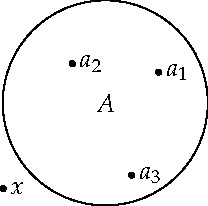
\includegraphics{sets-01-venn}
\end{defn}

As in the definition, it is typical to use upper-case letters ($A,B,C,\ldots$) for abstract sets and lower-case letters for their elements.\smallbreak

\emph{Venn diagrams} are useful for visualizing abstract sets. A set is represented by a region in the plane, with elements depicted by dots. The diagram in the definition represents a set $A$ comprising at least four elements $a_1,a_2,a_3$ and $x$. The element $y$ does not lie in $A$. 

\begin{example}{}{}
	Let $A$ be the set of (names of) US states. Then Michigan $\in A$ and Saskatchewan $\notin A$.
\end{example}

\begin{defn}{}{subset}
	Let $A$ and $B$ be sets.
	\begin{enumerate}
	  \item Sets are \emph{equal,} written $A=B$, if they have precisely the same elements.\par
	  \begin{minipage}[t]{0.74\linewidth}\vspace{-4pt}
	  	\item $A$ is a \emph{subset} of $B$, written $A\subseteq B$, if every element of $A$ is also an element of $B$.
	  	\item $A$ is a \emph{proper subset} of $B$ if $A\subseteq B$ and $A\neq B$. To stress this, we'd write $A\subsetneq B$. The Venn diagram on the right represents a proper subset. 
	  \end{minipage}
	  \hfill
	  \begin{minipage}[t]{0.25\linewidth}\vspace{-15pt}
			\flushright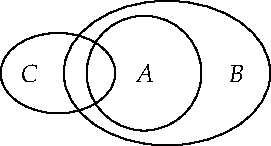
\includegraphics{sets-02-vennsubset}
	  \end{minipage}
	\end{enumerate}
\end{defn}

The following observations are simply translations of the definition:
\begin{enumerate}
  \item Equality: $A=B \iff A\subseteq B$ and $B\subseteq A$.
  \item Subset: $A\subseteq B \iff \bigl(x\in A\Longrightarrow x\in B\bigr) \iff \bigl(\forall x\in A, x\in B\bigr)$
  \item Not a subset: $A\nsubseteq B \iff \exists x\in A$ for which $x\notin B$.
\end{enumerate}


\boldsubsubsection{Roster \& Set-Builder Notation}

\emph{Roster notation} is the most basic way to describe the elements of a set: simply \emph{list} the elements in any order between curly brackets $\{\,,\,\}$.

\begin{example}{}{easysetnotation}
	Let $A$ be the set of (real number) solutions to the equation $2x^2-7x+3=0$ and let $B$ be the set of \emph{integer} solutions to the same equation. Since the polynomial factorizes as $(2x-1)(x-3)$, we see that $A=\{3,\frac 12\}$ and $B=\{3\}$. We could also write $A=\{\frac 12,3\}$ since \emph{order doesn't matter in roster notation.}	Moreover:
	\begin{itemize}
	  \item $A\nsubseteq B$ since $\frac 12\in A$ and $\frac 12\notin B$.
	  \item $B\subseteq A$ since 3 (the only element of $B$) lies in $A$. Indeed $B\subsetneq A$ is a  proper subset since $A\neq B$.
	\end{itemize}
\end{example}

Roster notation is ideal for small sets, but is of limited utility when trying to describe large sets. This is where our second notation rides to the rescue.\bigbreak

\emph{Set-builder notation} describes the elements of a set using some common property. Suppose $\cU$ is some (already understood) set and $P(x)$ is a propositional function with domain $\cU$, then
\[
	A:=\bigl\{x\in\cU:P(x)\bigr\} \tag{``$A$ is the set of $x$ in $\cU$ such that $P(x)$''}
\]
defines a set $A$ as \emph{the subset} of $\cU$ all of whose elements $x$ satisfy the property $P(x)$. A vertical separator $\mid$ is often used instead of a colon: we'll use both, though it might be essential in a given context to use one rather than the other for clarity.

\begin{examples}{}{}
\exstart Continuing Example \ref{ex:easysetnotation}, recall that $\R$ represents the set of real numbers and $\Z$ the set of integers. In set-builder notation, our solution sets may be written
	\[A=\bigl\{x\in\R:2x^2-7x+3=0\bigr\},\qquad B=\bigl\{x\in\Z:2x^2-7x+3=0\bigr\}\]
	In this case the qualifying proposition $P(x)$ is ``$2x^2-7x+3=0$.''
	\begin{enumerate}\setcounter{enumi}{1}
	  \item[]We can also express the fact that $B$ is a subset of $A$ in this notation (this time with a vertical separator),
	\[B=\bigl\{x\in A\bigm| x\in\Z\} \tag{``the set of elements $x$ in $A$ such that $x$ is an integer"}\]
	
	\item Let $X=\{2,4,6\}$ and $Y=\{1,2,5,6\}$. There are many options for how to write these in set-builder notation. For instance:
	\[
		X=\bigl\{n\in\Z:\tfrac 12n\in\{1,2,3\}\bigr\},\qquad Y=\bigl\{n\in\Z\bigm|1\le n\le 6\text{ and }n\neq 3,4\bigr\}
	\]
	We now practice the opposite skill by converting five sets from set-builder to roster notation.
	\begin{align*}
		&S_1=\bigl\{x\in X:x\text{ is divisible by 4}\bigr\}=\{4\}
		&&
		S_2=\bigl\{y\in Y:y\text{ is odd}\bigr\}=\{1,5\}
		\\
		&S_3=\bigl\{x\in X\bigm| x\in Y\bigr\}=\{2,6\}
		&&
		S_4=\bigl\{x\in X:x\notin Y\bigr\}=\{4\}
		\\
		&S_5=\bigl\{y\in Y\bigm| y\text{ is odd and $y-1\in X$}\}=\{5\}
	\end{align*}
	Can you find alternative descriptions in set-builder notation for the sets $S_1,\ldots,S_5$ above? Take your time getting used to this notation: the ability to translate between various descriptions of a set is \emph{crucial} to reading mathematics!
	
	\item Use the set $C=\{0,1,2,3,\ldots,24\}$ to describe $D=\{n\in\Z:n^2-3\in C\}$ in roster notation.\par
  Expand the criterion for membership in $D$:
  \[
  	n^2-3\in C\iff n^2\in\bigl\{3,4,5,\ldots,25,26,27\bigr\}
  \]
  Since $n$ must be an integer, it follows that $D=\{\pm 2,\pm 3,\pm 4,\pm 5\}$.
  
  \item To express $E=\{0,2,6,12,\ldots\}$ in set-builder notation we might spot a pattern and decide that
  \[
  	E=\bigl\{n\in\Z: n=m(m+1) \text{ for some integer }m\ge 0\bigr\}
  \]
  The problem is that we cannot guarantee our correctness! Perhaps the correct formula is
  \[
  	n=m(m+1)+m(m-2)(m-6)(m-12)
  \]
	In the first case the next term in the sequence is $4\cdot 5=20$, whereas in the second case it is $20+128=148$. For larger sets, the clarity afforded by set-builder notation is essential!

	\end{enumerate}
\end{examples}



\boldsubsubsection{Common Sets of Numbers}

We've used some of this notation already, and much of the rest should be familiar.% with much of it from your previous studies. Common sets of numbers are often written using the $\mathbb{B}${\scriptsize $\mathbb{LACKBOARD}$} $\mathbb{B}${\scriptsize $\mathbb{OLD}$} typeface.
\vspace{-2pt}

\begin{quote}\def\arraystretch{1.15}
\begin{tabular}{@{}ll}
	\emph{Natural numbers}&$\N=\bigl\{1,2,3,4,\ldots\bigr\}$ is the set of \emph{positive} integers.\\
	\emph{Integers}&$\Z=\bigl\{\ldots,-3,-2,-1,0,1,2,3,\ldots\bigr\}$.\\
	\emph{Rational numbers}&$\Q=\bigl\{\frac mn:m\in\Z\text{ and }n\in\N\bigr\} =\bigl\{\frac ab\bigm| a,b\in\Z\text{ and }b\neq 0\bigr\}$.\\
	\emph{Real numbers}&$\R$. Even a rudimentary definition is too involved for this text.\footnote{We simply assume the reader is comfortable with the idea of the real line where number corresponds to \emph{length.} A rigorous development of $\R$ is a matter for an upper-division \emph{analysis} course.}\\
	\emph{Complex numbers}&$\C=\bigl\{x+iy:x,y\in\R\bigr\}$ where $i^2=-1$. We won't use these.
\end{tabular}
\end{quote}

\begin{examples}{}{}
	\exstart For instance: \ $7\in\N$, \ $\pi\in\R$, \ $-\frac 79\notin\Z$, \ $\sqrt 2\notin\Q$ \ and \ $3+\sqrt 5i\in\C$.
	\begin{enumerate}\setcounter{enumi}{1}
	  \item The basic symbols can be decorated to make natural modifications. For example:
\vspace{-3pt}
		\begin{itemize}
		  \item $\N_0=\bigl\{0,1,2,3,4,\ldots\bigr\}=\Z^+_0=\bigl\{x\in\Z:x\ge 0\bigr\}$. Also called the \emph{whole numbers} ($\mathbb W$).
			\item $\Z_{\ge 5}=\bigl\{5,6,7,8,\ldots\bigr\} =\bigl\{x\in\Z:x\ge 5\bigr\}$ denotes the integers greater than or equal to 5.
		  \item $\R^+=\bigl\{x\in\R:x>0\bigr\}$ is the set of positive real numbers.
			\item $4\Z=\bigl\{\ldots,-8,-4,0,4,8,12,\ldots\bigr\} =\bigl\{x\in\Z: 4\mid x\bigr\}$ is the set\footnotemark{} of integer multiples of 4.\par
			This notation can be used for non-integer multiples, e.g. $\pi\Z=\bigl\{\ldots,-\pi,0,\pi,2\pi,\ldots\bigr\}$. 
			\item $2\Z+1=\bigl\{x\in\Z:x\equiv 1\pmod 2\bigr\}$ is the set of odd integers.
		\end{itemize}
		
		\item \emph{Intervals} are the most commonly encountered subsets of the real numbers. For instance:
\vspace{-3pt}
		\begin{itemize}
		  \item $[1,\pi]=\bigl\{x\in\R\bigm|1\le x\le \pi\bigr\}$ is a \emph{closed} interval 
		  \item $[-4,7.21)=\{x\in\R\bigm|-4\le x<7.21\}$ is a \emph{half-open} interval.
		  \item $(-\infty, \sqrt 2) =\{x\in\R\bigm|x<\sqrt 2\}$ is an \emph{infinite (open)} interval.
		\end{itemize}
	\end{enumerate}
\end{examples}

\footnotetext{Be careful here!---the colon is the ``such that" separator while $\mid$ denotes the property ``4 divides $x$.'' The unreadability of $\bigl\{x\in\Z\bigm| 4\mid x\bigr\}$ illustrates the benefit of having two separator symbols to choose from.}

\goodbreak

In view of the natural subset relationships $\N\subsetneq\Z\subsetneq\Q\subsetneq\R\subsetneq\C$, we consider a simple result.

\begin{lemm}{Transitivity of Subset}{subsettrans}
	Suppose $A\subseteq B$ and $B\subseteq C$. Then $A\subseteq C$.
\end{lemm}

\begin{proof}
	Think back to the criteria following Definition \ref{defn:subset}. Suppose $A\subseteq B$ and $B\subseteq C$. Then
	\[
		x\in A \overset{(A\subseteq B)}{\implies} x\in B\overset{(B\subseteq C)}{\implies} x\in C
	\]
	We conclude that $A\subseteq C$.
\end{proof}

Compare this to Exercise \ref*{sec:prop}.\ref{exs:iftransitive}: if we translate each subset relation into an implication, the proof structure is $(x\in A\Rightarrow x\in B)\wedge (x\in B\Rightarrow x\in C)\Longrightarrow (x\in A\Rightarrow x\in C)$. This is typical of basic results about sets: after translation, the theorem reduces to one of the standard rules of logic.



\boldsubsubsection{Cardinality and the Empty Set}

It is helpful to introduce some terminology to describe the \emph{size} of a set.

\begin{defn}{}{}
	A \emph{finite set} contains only a finite number of elements: this number is its \emph{cardinality,} written $\nm A$. A set with infinitely many elements is said to be an \emph{infinite set.}\par
	The symbol $\emptyset$ denotes the \emph{empty set}: a set containing no elements (cardinality zero: $\nm\emptyset=0$).
\end{defn}



\begin{examples}{}{}
	\exstart Let $A=\bigl\{1,3,\pi,\sqrt 2,103\bigr\}$, then $\nm A=5$.
	\begin{enumerate}\setcounter{enumi}{1}
		\item Let $B=\bigl\{4,\{1,2\},\{3\}\bigr\}$. The elements of $B$ are $4$, $\{1,2\}$ and $\{3\}$, therefore $\nm B=3$. It doesn't matter that the \emph{element} $\{1,2\}\in B$ is also a set!\par
		\begin{minipage}[t]{0.59\linewidth}\vspace{-5pt}
			\item Recall some basic trigonometry:
			\[
				\left\{x\in[0,4\pi]:\cos x=\frac 12\right\}=\left\{\frac{\pi}3,\frac{5\pi}3,\frac{7\pi}3,\frac{11\pi}3\right\}
			\]
			has cardinality 4.
		\end{minipage}
		\hfill
		\begin{minipage}[t]{0.4\linewidth}\vspace{-10pt}
			\flushright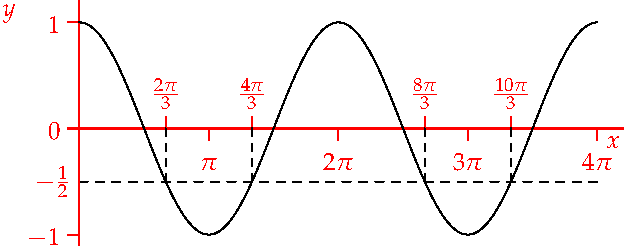
\includegraphics{sets-03-cos}
		\end{minipage}
		
		\item There are many representations of the empty set: for example
		\[
			\emptyset =\bigl\{x\in\R:x^2=-1\bigr\} = \bigl\{x\in\N:x^2+3x+2=0\bigr\}=\bigl\{n\in\N:n<0\bigr\}
		\]
		In general, if $X$ is any set and $P(x)$ is false for all $x\in X$, then\footnotemark{} $\emptyset=\bigl\{x\in X:P(x)\bigr\}$.
	\end{enumerate}
\end{examples}

\footnotetext{In some formalizations of set theory, the existence of the empty set is an axiom: an assumption made without proof. Provided one accepts that set-builder notation always defines a set---this is itself an axiom!---and that at least one set $X$ exists, the empty set may be \emph{defined} as in the example: a suitable property $P(x)$ might be something like ``$x\notin\{x\}$.''}


Cardinality is a very simple concept for finite sets; if $B$ is finite, so is any subset, and we have
\[
	A\subseteq B\implies \nm A\le \nm B
\]
For infinite sets, cardinality is more subtle. We'll return to this issue and uncover some of the bizarre and fun consequences of infinite cardinalities in Chapter \ref{chap:cantor}.
\bigbreak

We finish with a couple of simple results regarding the empty set.

\begin{lemm}{}{}
Let $A$ be a set.
\begin{enumerate}
  \item If $\nm A=0$, then $A=\emptyset$. The empty set is \emph{the unique set} with zero cardinality.
  \item $\emptyset\subseteq A$ and $A\subseteq A$
\end{enumerate}
\end{lemm}

\begin{proof}
	Think about the claim $\emptyset\subseteq A$: by the observations following Definition \ref{defn:subset}, this means
	\[
		x\in\emptyset\implies x\in A
	\]
	This is true (for any set $A$!) since there are no elements $x$ satisfying the hypothesis.\footnotemark{}
	\begin{enumerate}
 	 \item Suppose $A$ has cardinality zero. Repeating and combining with the above observation, we see that $\emptyset\subseteq A$ and $A\subseteq\emptyset$. We conclude that $A=\emptyset$.
 	 \item We already know that $\emptyset\subseteq A$. For the second part, simply observe that
 	 $x\in A\implies x\in A$.\qedhere
\end{enumerate}
\end{proof}

\footnotetext{If $P(x)$ is always false, then $(\forall x)\ P(x)\Longrightarrow Q(x)$ is true. This is called a \emph{vacuous} (empty) theorem.}

% 
% 
% \begin{examples}{}{}
% 	\begin{enumerate}\setcounter{enumi}{1}
%   \item Are the following sets equal?
%   \[E=\{n^2+2\in\Z:\text{$n$ is an odd integer}\},\qquad F=\{n\in\Z:n^2+2\text{ is an odd integer}\}.\]
%   It may help to first construct a table listing some of the values of $n^2+2$:
%   \[\begin{array}{c|c|c}
%   n&n^2&n^2+2\\\hline
%   \pm 1&1&3\\
%   \pm 3&9&11\\
%   \pm 5&25&27\\
%   \pm 7&49&51\\
%   \pm 9&81&83\\[-5pt]
%   \vdots&\vdots&\vdots
%   \end{array}\]
%   The set $E$ consists of those integers of the form $n^2+2$ where $n$ is an odd integer. By the table,
%   \[E=\{3,11,27,51,83,\ldots\}.\]
%   On the other hand, $F$ includes all those integers $n$ such that $n^2+2$ is odd. It is easy to see that
%   \[n^2+2\text{ is odd}\iff n^2\text{ is odd}\iff n\text{ is odd.}\]
%   Thus $F$ is simply the set of all odd integers:
%   \[F=\{\pm 1,\pm 3,\pm 5,\pm 7,\ldots\}=2\Z+1.\]
%   Plainly the two sets are not equal.
% 
%   \item $\{x\in\R:x^2-1=0\}\subseteq \{y\in\R:y^2\in\N\}$.\\
%   To make sense of this relationship, convert to roster notation: we obtain
%   \[\{-1,1\}\subseteq\{\pm\sqrt 1,\pm\sqrt 2,\pm\sqrt 3,\pm\sqrt 4,\ldots\}.\]
%   \item If $m$ and $n$ are positive integers, then $m\Z\subseteq n\Z\iff n\mid m$. Make sure you're comfortable with this! For example, $4\Z\subseteq 2\Z$ since every multiple of 4 is also a multiple of 2.
% \end{enumerate}
% \end{examples}


% \paragraph{Self-test Questions}
% 
% \begin{enumerate}
%   \item True or false: An open interval contains its endpoints.
%   \item True or false: $\{x\in\R:x^2<0\}$ is a representation of the empty set.
%   \item True or false: $\{x\in\Z:x\in[0,4)\}=\{0,1,2,3,4\}$.
% \end{enumerate}


\begin{exercises}{}{}
	A reading quiz and several questions with linked video solutions can be found \href{http://www.math.uci.edu/~ndonalds/math13/selftest/4-1-subset.html}{online}.


% Write the set $A=\{x\in\R:x^2+3x+2=0\}$ in roster notation.\\[5pt]
% 	We are looking for the set of all real number solutions to the quadratic equation $x^2+3x+2=0$. A simple factorization tells us that $x^2+3x+2=(x+1)(x+2)$, whence $A=\{-1,-2\}$.

	\begin{enumerate}
	  \item Describe the following sets in roster notation: that is, list their elements.
		\begin{enumerate}
		  \item \makebox[215pt][l]{$\bigl\{x\in\N:x^2\le 3x\bigr\}$\hfill (b)} \ $\bigl\{n\in\{0,1,2,3,\ldots,19\}:n+3\equiv 5\spmod 4\bigr\}$
		  \setcounter{enumii}{2}
		  \item \makebox[215pt][l]{$\bigl\{n\in\{-2,-1,0,1,\ldots,23\}:4\mid n^2\bigr\}$\hfill (d)} \ $\bigl\{x\in \frac 12\Z: 0\le x\le 4\text{ and }4x^2\in 2\Z+1\bigr\}$
		  \setcounter{enumii}{4}
		  \item $\bigl\{y\in\R:y=x^2\text{ for some $x\in\R$ with } x^2-3x+2=0\bigr\}$
		\end{enumerate}
			
			
		\item Describe the following sets in set-builder notation (\emph{look for a pattern}).
		\begin{enumerate}
		  \item \makebox[180pt][l]{$\bigl\{\ldots,-3,0,3,6,9,\ldots\bigr\}$\hfill (b)} \ $\bigl\{-3,1,5,9,13,\ldots\bigr\}$
		  \setcounter{enumii}{2}
		  \item $\bigl\{1,\frac 13,\frac 17,\frac 1{15},\frac 1{31},\ldots\bigr\}$
		\end{enumerate}
		  
	
	  \item Each of the following sets of real numbers is a single interval. Determine the interval.
		\begin{enumerate}
		  \item \makebox[180pt][l]{$\bigl\{x\in\R:x>3\text{ and }x\le 17\bigr\}$\hfill (b)} \ $\bigl\{x\in\R:x\nleq 3\text{ or }x\le 17\bigr\}$
		  \setcounter{enumii}{2}
		  \item \makebox[180pt][l]{$\bigl\{x^2\in\R:x\neq 0\bigr\}$ \hfill (d)} \ $\bigl\{x\in\R^-:x^2\ge 16\text{ and }x^3\le 27\bigr\}$
		\end{enumerate}
			
			
		\item Is the set $\{x\in\Z:-1\le x<43\}$ finite or infinite? If finite, what is its cardinality?
				
		
		%\item Compare the sets $A=\{3x\in\Z:x\in 2\Z\}$ and $B=\{x\in\Z:x\equiv 12\pmod 6\}$. Are they equal?
			
			
		\item What is the cardinality of the set $\Bigl\{\emptyset,\bigl\{\emptyset\bigr\},\bigl\{\emptyset,\{\emptyset\}\bigr\}\Bigr\}$? \ What are its elements?
		
		\item Let $A=\emptyset$, \ $B=\{A\}$, \ $C=\bigl\{\{A\}\bigr\}$ \ and \ $D=\bigl\{A,\{0\},\{0,1\}\bigr\}$.\par
	  Answer the following true or false:
	  \begin{enumerate}
	    \item \makebox[80pt][l]{$0\in A$\hfill (b)} \ \makebox[80pt][l]{$A\in B$\hfill (c)} \ \makebox[80pt][l]{$A\in C$\hfill (d)} \ \makebox[80pt][l]{$B\in C$ \hfill (e)} \ $A\in D$
	    \setcounter{enumii}{5}
	    \item \makebox[80pt][l]{$B\in D$\hfill (g)} \ \makebox[80pt][l]{$0\in D$\hfill (h)} \ \makebox[80pt][l]{$\{0\}\in D$\hfill (i)} \ $\{1\}\in D$
	  \end{enumerate}
	  
	  
	  \item List all the \emph{proper} subsets of $\{1,2,3\}$.
	  
	    
		\goodbreak
	   
		   
		\item Let $A,B,C,D$ be the following sets:
	  \begin{align*}
	  	&A=\{-4,1,2,4,10\}
	  	&&B=\bigl\{m\in\Z:\nm m\le 12\bigr\}\quad \text{(\emph{absolute value of $m$})}\\
	  	&C=\bigl\{n\in\Z:n^2\equiv 1\spmod 3\bigr\}
	  	&&D=\bigl\{t\in\Z:t^2+3\in [4,20)\bigr\}  
	  \end{align*}
	  Of the 12 subset relations $A\subseteq B$,\ $A\subseteq C,\ldots, D\subseteq C$, which are true and which false?
	  
	  \item Let $A=\bigl\{1,2,\{1,2\},\{3\}\bigr\}$ and $B=\{1,2\}$. Answer the following true or false:
	  \begin{enumerate}
	    \item \makebox[100pt][l]{$B\in A$\hfill (b)} \ \makebox[100pt][l]{$B\subseteq A$\hfill (c)} \ \makebox[100pt][l]{$3\in A$\hfill (d)} \ $\{3\}\subseteq A$
	    \setcounter{enumii}{4}
	    \item \makebox[100pt][l]{$\{3\}\in A$\hfill (f)} \ \makebox[100pt][l]{$\emptyset\subseteq A$\hfill (g)} \ $\emptyset\in A$
	  \end{enumerate}
	  
	  \item Let $A=\{0,2,4,6,8,10\}$. Write the set $B=\{X\subseteq A:|X|=2\}$ in roster notation.
	  
	    
	  \item\begin{enumerate}
	    \item Suppose $A\subseteq B\subseteq C\subseteq A$. Show that $A=B=C$.
	    \item Is it possible for sets $A,B,C$ to satisfy $A\subsetneq B\subseteq C\subseteq A$? Why/why not?
	  \end{enumerate}

	
		\item Let $A=\{\text{1,2,3,4}\}$, and let $B =\bigl\{\{x,y\}:x,y\in A\bigr\}$.
		\begin{enumerate}
	  	\item Describe $B$ in roster notation (\emph{what happens when $x=y$?}).
			\item Find the cardinalities of the following sets:
			\[
				C=\Bigl\{\bigl\{x,\{y\}\bigr\}:x,y\in A\Bigr\}
				\quad\text{and}\quad
				D=\biggl\{\Bigl\{\bigl\{x,\{y\}\bigr\}:x,y\in A\Bigr\}\biggr\}
			\]
		\end{enumerate}
  
  
  	\item Let $A=\{x\in\R:x^3+x^2-x-1=0\}$ and $B=\{x\in\R:x^4-5x^2+4=0\}$. Are either of the relations $A\subseteq B$ or $B\subseteq A$ true? Explain.
  
  
  	\item For which real numbers $x>0$ do we have $[0,x]\subsetneq[0,x^2]$? Prove your assertion.
  
  
  	\item Let $m,n\in\N$. Prove: $m\Z\subseteq n\Z\iff n\mid n$.

  
  	\item\label{ex:mirrored} Given $A\subseteq\Z$ and $x\in\Z$, we say that $x$ is $A$-mirrored if and only if $-x\in A$. Also define
  	\[
			M_A:=\bigl\{x\in\Z: x\text{ is $A$-mirrored}\bigr\}
		\]
		\begin{enumerate}
	  	\item What does it mean for $x$ \emph{not} to be $A$-mirrored?
	  	\item Find $M_B$ given $B=\{0,1,-6,-7,7,100\}$.
	  	\item Assume that $A \subseteq\Z$ is closed under addition: for all $x,y\in A$, we have $x+y\in A$. Show that $M_A$ is closed under addition.
	  	\item In your own words, under which conditions is $A=M_A$?
		\end{enumerate}

  \item Define the set $[1]=\bigl\{x\in\Z: x\equiv 1\spmod 5\bigr\}$.
		\begin{enumerate}
		  \item Describe the set $[1]$ in roster notation.
		  \item Compute the set $M_{[1]}$, as defined in Exercise \ref{ex:mirrored}. Is $M_{[1]}$ equal to $[1]$?
			\item Now consider the set $[10]=\{x\in\Z:x\equiv 10\spmod 5\}$. Are the sets $[10]$ and $M_{[10]}$ equal? Prove or disprove.
  	\end{enumerate}


     % \item (Hammack's \href{http://www.people.vcu.edu/~rhammack/BookOfProof/}{\emph{Book of Proof}}, Section 1.3, Exercise 6)
%List all subsets of $\{\R,\Q,\N\}$.
    

		\item Consider the set $A=\{a,b,c,d\}$. 
    \begin{enumerate}
      \item Of each cardinality 0, 1, 2, 3 and 4, how many subsets has $A$? Is there a pattern?
        
      \item Completely expand the polynomial $(1 + x)^4$. What do you notice about the coefficients? 
    \end{enumerate}

	\end{enumerate}
\end{exercises}

\clearpage



\subsection{Unions, Intersections and Complements}\label{sec:union}

In this section we construct new sets from old, modeled precisely on the logical concepts of \emph{and, or,} and \emph{not} (compare Definition \ref{defn:andornot}). 


\begin{defn}{}{unionint}
	Let $\cU$ be a (universal) set,\footnotemark{} and suppose $A,B$ are subsets of $\cU$.
	\begin{enumerate}\itemsep0pt
		\item The \emph{union} of $A$ and $B$ is the set of elements in $A$ or $B$:
		\[
			\makebox[210pt][l]{$A\cup B:=\bigl\{x\in\cU:x\in A\text{ or }x\in B\bigr\}$\hfill} (x\in A\cup B\iff x\in A\text{ or }x\in B)
		\]
		\item The \emph{intersection} of $A$ and $B$ is the set of elements in both $A$ and $B$:
		\[
			\makebox[210pt][l]{$A\cap B:=\bigl\{x\in\cU:x\in A\text{ and }x\in B\bigr\}$\hfill} (x\in A\cap B\iff x\in A\text{ and }x\in B)
		\]
		We say that $A$ and $B$ are \emph{disjoint} if $A\cap B=\emptyset$.
	  \item The \emph{complement} of $A$ is the set of all elements not in $A$:
		\[
			\makebox[210pt][l]{$\comp A:=\bigl\{x\in\cU:x\notin A\bigr\}$ \hfill} (x\in\comp A\iff x\notin A \ (\text{and }x\in\cU))
		\]
		This can be read ``$B$ minus $A$'', indeed some authors write $B-A$. Similarly $\comp A=\cU\setminus A$, etc.
		\item The \emph{complement of $A$ relative $B$} is the set of elements in $B$ which are not in $A$:
		\[
			\makebox[210pt][l]{$B\setminus A:=B\cap \comp A=\bigl\{x\in B:x\notin A\bigr\}$\hfill} (x\in B\setminus A\iff x\in B\text{ and } x\notin A)
		\]
	\end{enumerate}
	
	\begin{center}
		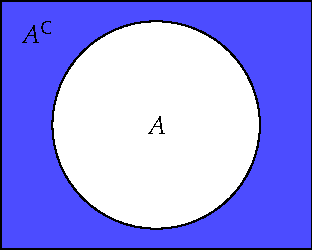
\includegraphics{sets-05-venncomp}
		\qquad\qquad
		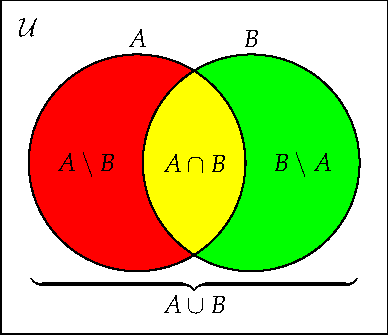
\includegraphics{sets-04-vennunion}
	\end{center}
\end{defn}

\footnotetext{Of which everything else will be a subset. This is needed particularly for complements, but more generally is required to invoke set-builder notation. In certain contexts, the universal set is naturally assumed: $\cU=\R$ makes sense if you are working within the real numbers, $\cU=\Z$ if doing modular arithmetic.}

In the Venn diagrams, the outer box depicts the universal set $\cU$. Though it doesn't constitute a proof, the diagram makes certainly suggests that
\[
	A=(A\setminus B)\cup (A\cap B) \quad\text{and}\quad B=(B\setminus A)\cup(A\cap B)
\]
Observe the notational similarity with logic: $\cup$ looks a bit like $\vee$ (OR); $\cap$ like $\wedge$ (AND).

\begin{examples}{}{}
	\exstart Let $\cU=\{1,2,3,4,5\}$, $A=\{1,2,3\}$, and $B=\{2,3,4\}$. Then
	\begin{align*}
		&\comp A=\{4,5\} &&\comp B=\{1,5\} &&B\setminus A=\{4\} &&A\setminus B=\{1\}\\
		&A\cup B=\{1,2,3,4\} &&A\cap B=\{2,3\} &&A\cap\comp B=\{1\} &&\comp A\cup\comp B=\{1,4,5\}
	\end{align*}
	
	\goodbreak
		
	\begin{enumerate}\setcounter{enumi}{1}
		\item Using interval notation, let $\cU=[-4,5]$, \ $A=[-3,2]$, \ and \ $B=[-4,1)$. Then\par
% 		\begin{align*}
% 			&\comp A=[-4,-3)\cup (2,5] &&\comp B=[1,5] &&A\cup B=[-4,2] \\
% 			&A\setminus B=[1,2] &&B\setminus A=[-4,-3) &&A\cap B=[-3,1) 
% 		\end{align*}
% 		\vspace{-24pt}
% 		\begin{center}
% 		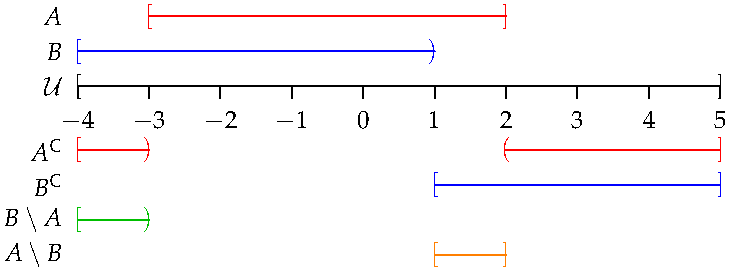
\includegraphics[width=0.7\textwidth]{sets-13-intervalex}
% 		\end{center}
% 		\vspace{-13pt}
		\begin{minipage}[t]{0.3\linewidth}\vspace{-13pt}
			\begin{gather*}
			\comp A=[-4,-3)\cup (2,5]\\
			\comp B=[1,5]\\
			A\setminus B=[1,2]\\
			B\setminus A=[-4,-3)\\
			A\cup B=[-4,2]\\
			A\cap B=[-3,1) 
			\end{gather*}
		\end{minipage}
		\hfill
		\begin{minipage}[t]{0.69\linewidth}\vspace{0pt}
			\flushright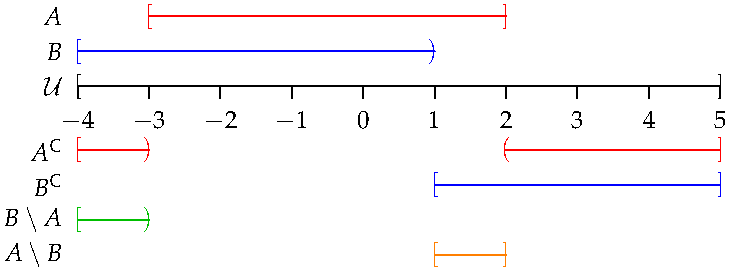
\includegraphics[scale=0.8]{sets-13-intervalex}
		\end{minipage}
		\smallbreak
		While you should be comfortable with these just from the picture, for practice it is worth trying algebraic arguments. In particular, note how $\comp A$ relies on de Morgan's law (Theorem \ref{thm:demorgan}):
		\begin{align*}
			x\in \comp A&\iff x\notin A\iff \neg\bigl(x\in A\bigr) \iff\neg\bigl(-3\le x \text{ and }x\le 2\bigr)\\
			&\iff x<-3\text{ or }x>2 \tag{de Morgan}\\
			&\iff x\in[-4,-3)\cup (2,5] \tag{remember that $x\in\cU$ always!}
		\end{align*}
		
		\item Let $A=(-\infty,3)$ and $B=[-2,\infty)$ in interval notation. Then $A\cup B=\R$ and $A\cap B=[-2,3)$.
	\end{enumerate}
\end{examples}


For the remainder of this section, we summarize the basic rules of set algebra.

\begin{thm}{Union/intersection rules}{setbasic}
	Let $A,B,C$ be sets. Then:
	\begin{enumerate}\itemsep2pt
		\item $\emptyset\cup A=A$ \ and \ $\emptyset\cap A=\emptyset$
		\item $A\cap B\subseteq A\subseteq A\cup B$
		\item $A\cup B=B\cup A$ \ and \ $A\cap B=B\cap A$
		\item $A\cup (B\cup C)=(A\cup B)\cup C$ \ and \ $A\cap (B\cap C)=(A\cap B)\cap C$
		\item $A\cup A=A\cap A=A$
		\item $A\subseteq B\Longrightarrow A\cup C\subseteq B\cup C$ \ and \ $A\cap C\subseteq B\cap C$
	\end{enumerate}
\end{thm}

If you don't believe a result, try \emph{visualizing} it using a Venn diagram. The basic proof strategy is the same for all parts: convert each statement into propositions (Definition \ref{defn:unionint} parentheses) and use what you know from basic logic (e.g., Theorem \ref{thm:demorgan} and page \pageref{pg:asidelogicalgebra}). We prove part 2 and half of part 6, leaving some of the rest to the Exercises.

\begin{proof}
\begin{enumerate}
  \item[2.] There are two results here: $A\cap B\subseteq A$ and $A\subseteq A\cup B$. We prove separately, with some commentary on the side.
	\begin{enumeratea}
		\item Suppose $x\in A\cap B$.\hfill(Goal: want to prove $x\in A\cap B\Rightarrow x\in A$)\par
		Then $x\in A$ and $x\in B$.\hfill(Definition of intersection)\par
		Plainly $x\in A$. We conclude that $A\cap B\subseteq A$\hfill(Definition of subset)
		\item Suppose $y\in A$.\hfill(Goal: prove $y\in A\Rightarrow y\in A\cup B$)\par
		Then ``$y\in A$ or $y\in B$'' is true, whence $y\in A\cup B$.\hfill(Definition of union/or)\par
	  We conclude that $A\subseteq A\cup B$.
	\end{enumeratea}
	
	\goodbreak
	
	\item[6.] (first half)\lstsp Suppose $A\subseteq B$. We wish to prove that $x\in A\cup B\Longrightarrow x\in A\cup C$. However,
	\begin{align*}
		x\in A\cup C&\implies x\in A\text{ or }x\in C\tag{definition of union}\\
		&\implies x\in B\text{ or }x\in C\tag{since $A\subseteq B$}\\
		&\implies x\in B\cup C \tag*{\qedhere}
	\end{align*}
\end{enumerate}
\end{proof}



The next batch of rules describe how complements interact with other set operations: parts 1 and 2 are \emph{de Morgan's laws for sets}; unsurprisingly, their proofs depend on the corresponding laws of logic.


\begin{thm}[lower separated=false, sidebyside, sidebyside align=top seam, sidebyside gap=0pt, righthand width=0.4\linewidth]{Complement rules}{setcomp}
	Let $A,B$ be sets. Then:
	\begin{enumerate}\itemsep2pt
		\item $\comp{(A\cap B)}=\textcolor{blue}{\comp A}\cup \textcolor{red}{\comp B}$ (see picture)
		\item $\comp{(A\cup B)}=\comp A\cap \comp B$
		\item $\smash[t]{\comp{(\comp A)}}=A$
		%\item $A\setminus B=A\cap\comp B$
		\item $A\subseteq B\iff \comp B\subseteq \comp A$
	\end{enumerate}
	\tcblower
	\flushright
	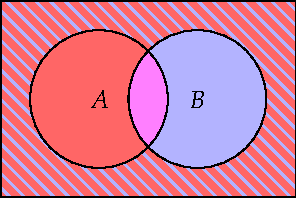
\includegraphics[scale=1]{sets-08-venndemorgan2}
\end{thm}

% \begin{proof}[Proof of 1.]
% We start by trying to show that the left hand side is a subset of the right hand side.
% \begin{align*}
% x\in\comp{(A\cap B)}&\implies x\notin A\cap B\\
% &\implies x\text{ is not a member of \emph{both} $A$ and $B$}\\
% &\implies x\text{ is not in \emph{at least one} of $A$ and $B$}\\
% &\implies x\notin A\text{ or }x\notin B\\
% &\implies x\in\comp A\text{ or }x\in\comp B\\
% &\implies x\in\comp A\cup\comp B
% \end{align*}
% With a little thinking, we realize that all of the $\Longrightarrow$ arrows may be replaced with if and only if arrows $\Longleftrightarrow$ without compromising the argument. We've therefore shown that the sets $\comp{(A\cap B)}$ and $\comp A\cup \comp B$ have the same elements, and are thus equal.
% \end{proof}


\begin{proof}
	We prove only part 1. As before, the natural approach is to restate the result using propositions.
	\begin{align*}
		x\in\comp{(A\cap B)}&\iff \neg\bigl(x\in A\cap B\bigr) \iff \neg\bigl(x\in A\ \text{ and }\  x\in B\bigr)\\
		&\iff \neg\bigl(x\in A\bigr)\ \text{ or }\ \neg\bigl(x\in B\bigr) \tag*{(de Morgan's first law of logic)}\\
		&\iff x\in\comp A\ \text{ or }\ x\in\comp B\\
		&\iff x\in\comp A\cup\comp B\tag*{\qedhere}
	\end{align*}
\end{proof}

Our final pair of results describe the interaction of unions and intersections.\par

\begin{thm}[lower separated=false, sidebyside, sidebyside align=top seam, sidebyside gap=0pt, righthand width=0.3\linewidth]{Distributive laws}{setdist}
	For any sets $A,B,C$:
	\begin{enumerate}\setlength{\itemsep}{2pt}
		\item $A\cap(B\cup C)=(A\cap B)\cup(A\cap C)$
		\item $A\cup(B\cap C)=(A\cup B)\cap(A\cup C)$
	\end{enumerate}
	The Venn diagram illustrates the second result: think about adding the colored regions.
	\tcblower
	\flushright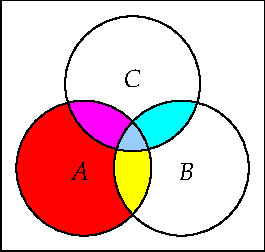
\includegraphics{sets-07-venndist}
\end{thm}


% 
% \begin{proof}
% \begin{itemize}
%   \item[($\subseteq$)] Let $x\in A\cup (B\cap C)$. Then $x\in A$ or $x\in B\cap C$. There are two cases:
%   \begin{itemize}
%     \item[(a)] If $x\in A$, then $x\in A\cup B$ and $x\in A\cup C$ by Theorem \ref{thm:setbasic}, part 2.
%     \item[(b)] If $x\in B\cap C$, then $x\in B$ and $x\in C$. It follows that $x\in A\cup B$ and $x\in A\cup C$, again by Theorem \ref{thm:setbasic}.
%   \end{itemize}
%   In both cases $x\in (A\cup B)\cap(A\cup C)$.
%   \item[($\supseteq$)] Let $y\in (A\cup B)\cap(A\cup C)$. Then $y\in A\cup B$ and $y\in A\cup C$. There are again two cases:
%   \begin{itemize}
%     \item[(a)] If $y\in A$, then we are done, for then $y\in A\cup (B\cap C)$.
%     \item[(b)] If $y\notin A$, then $y\in B$ and $y\in C$. Hence $y\in B\cap C$. In particular $y\in A\cup (B\cap C)$.
%   \end{itemize}
%   In both cases $y\in A\cup (B\cap C)$.\qedhere
% \end{itemize}
% \end{proof}


\begin{proof}
	We prove only the first result.
	\begin{align*}
		x\in A\cap(B\cup C) &\iff x\in A\text{ and }x\in B\cup C\\
		&\iff x\in A \text{ and }\bigl(x\in B\text{ or }x\in C\bigr)\\
		&\iff \bigl(x\in A \text{ and }x\in B\bigr)\text{ or }\bigl(x\in A\text{ and }x\in C\bigr) \tag{distributive law, page \pageref{pg:asidelogicalgebra}}\\
		&\iff x\in A\cap B\text{ or }x\in A\cap C\\
		&\iff x\in (A\cap B)\cup(A\cap C)\tag*{\qedhere}
	\end{align*}
\end{proof}

\goodbreak

% \paragraph{Self-test Questions}
% 
% \begin{enumerate}
%   \item The set operations of complement, union and intersection are based, respectively, on the logical constructions \underline{\phantom{not\quad}}, \underline{\phantom{or\quad}}, and \underline{\phantom{and\quad}}.
%   \item The result $\comp{(A\cup B)}=\comp A\cap\comp B$ is one of \underline{\phantom{De Morgan's laws\qquad}}.
%   \item True or false: if $A$ and $B$ are finite sets, then $A\cap B$ has strictly smaller cardinality than $A$.
%   \item True or false: if $A$ is a finite set, then $\comp A$ is a finite set.
%   \item True of false: if $A$ and $B$ are finite sets, then $\nm{A\cup B}\le\max(\nm A,\nm B)$.
% \end{enumerate}

\begin{exercises}{}{}
	A reading quiz and several questions with linked video solutions can be found \href{http://www.math.uci.edu/~ndonalds/math13/selftest/4-2-union.html}{online}.
	
\begin{enumerate}
  \item Describe each set in as simple a manner as you can: e.g.,
	\[
		\bigl\{x\in\R:(x^2>4\text{ and } x^3<27)\text{ or } x^2=15\bigr\}=(-\infty,-2)\cup (2,3)\cup\{\sqrt{15}\}
	\]
  \begin{enumerate}
	 	\item $\bigl\{x\in\R:x^2\neq x\bigr\}$
		\item $\bigl\{x\in\R:x^3-2x^2-3x\le 0\text{ or }x^2=4\bigl\}$
		\item $\bigl\{y\in\R:\exists x\in\R \text{ with }y=x^2 \text{ and }x\neq 1\bigl\}$
		\item $\bigl\{z\in\Z:z^2\text{ is even and $z^3$ is odd}\bigl\}$
		\item $\bigl\{y\in 3\Z+2:y^2\equiv 1\spmod 3\bigl\}$
	\end{enumerate}
  
  \item Let $A=\{1,3,5,7,9\}$, $B=\{1,4,7,10\}$ and $\cU=\{1,2,\ldots,10\}$. What are the following sets?
    \begin{enumerate}
	  	\item \makebox[100pt][l]{$A\cap B$\hfill (b)} \ \makebox[100pt][l]{$A\cup B$\hfill (c)} \ \makebox[100pt][l]{$B\setminus A$\hfill (d)} \ $\comp A$ 
	  	\setcounter{enumii}{4}
	  	\item \makebox[100pt][l]{$\comp{(A\setminus B)}$ \hfill (f)} \ \makebox[100pt][l]{$\comp A\cap \comp B$\hfill (g)} \ $(A\cup B)\setminus (A\cap B)$
		\end{enumerate}
	
  	
% 	\item Consider Theorems \ref{thm:setbasic} and \ref{thm:setdist}. In all seven results, replace the symbols in the first row of the following table with those in the second. Which of the results seem familar? Which are false?
% \[\begin{array}{c|c|c|c|c}
% \emptyset&A,B,C\text{ sets}&\cup&\cap&\subseteq\\\hline
% 0&A,B,C\in\N_0&+&\cdot&\le
% \end{array}\]

	%\item Prove that $B\setminus A=B\iff A\cap B=\emptyset$.
	
	\item Give formal proofs of the following parts of Theorems \ref{thm:setbasic}, \ref{thm:setcomp} and \ref{thm:setdist}. %With practice you should be able to prove \emph{all} of parts of these theorems \emph{without} looking at the arguments in the notes!
	\begin{enumerate}
	  \item \makebox[180pt][l]{$\emptyset\cap A=\emptyset$\hfill (b)} \ $A\cap (B\cap C)=(A\cap B)\cap C$
	  \setcounter{enumii}{2}
		\item \makebox[180pt][l]{$\comp{(\comp A)}=A$\hfill (d)} \ $A\cup(B\cap C)=(A\cup B)\cap(A\cup C)$
		\setcounter{enumii}{4}
		\item $A\subseteq B\iff \comp B\subseteq \comp A$
	\end{enumerate}


	\item By showing that each side is a subset of the other, give a formal proof of the set identity
	\[
		A=(A\setminus B)\cup (A\cap B)
	\]
	Now repeat your argument using only results from set algebra (Theorems \ref{thm:setcomp} and \ref{thm:setdist}).
	
	
	\item Prove that $A\cup B=A\iff B\subseteq A$.
	
	
	\item Prove that $\comp{(A\cap B\cap C)}=\comp A\cup\comp B\cup\comp C$
	
		
	  \item Prove or disprove the following conjectures (\emph{Hint: revisit Section \ref{sec:proof2}}).
	  \begin{enumerate}
	    \item $\exists x\in\R\setminus\Q$ such that $x^2\in\Q$.
	    \item $\forall x\in\R\setminus\Q$ we have $x^2\in\Q$.
		\end{enumerate}
	
	
	  \item Let $A\subseteq\R$, and let $x\in\R$. We say that $x$ is \emph{far away} from the set $A$ if and only if:
	  \[
	  	\exists d>0 \ \text{ such that } A\cap[x-d,x]=\emptyset
	  \] 
		If this does not happen, we say that $x$ is \emph{close to} $A$.
  	\begin{enumerate}
			\item Draw a picture of a set $A$ and elements $x,y$ such that $x$ is \emph{far away} from and $y$ is \emph{close to} $A$. 
			\item State the meaning of ``$x$ is close to $A$'' \ (negate ``$x$ is far away from $A$'').
			%\item Let $A=\{1,2,3\}$. Show that $x=4$ is \emph{far away} from $A$ using the definition.
			%\item Let $A=\{1,2,3\}$. Show that $x=1$ is \emph{close} to $A$.
			\item Let $A=\{1,2,3\}$.
			\begin{enumerate}
			  \item Show that $x=4$ is \emph{far away} from $A$ using the definition.
				\item Let $A=\{1,2,3\}$. Show that $x=1$ is \emph{close} to $A$.
			\end{enumerate}
			\item For general $A\subseteq\R$, show that if $x\in A$, then $x$ is \emph{close} to $A$.
			\item Let $A=(a,b)$ be a bounded interval. Is the end-point $a$ \emph{far away} from $A$?  What about $b$?
  	\end{enumerate}
  	
	\end{enumerate}

\end{exercises}

\clearpage

\iffalse

\subsection{Introduction to Functions}\label{sec:func1}

Sets become a lot more useful and interesting once you start transforming their elements! This is accomplished using \emph{functions.} In this section we introduce some basic concepts and notation, at least some of which should already be familiar. A formal definition will be given in Chapter \ref{chap:relations}, but for the present the following will suffice.

\begin{defn}{}{}
	Let $A$ and $B$ be sets. A \emph{function} $f$ with \emph{domain} $A$ and \emph{codomain} $B$ is a rule that assigns to each input $a\in A$ a single output $b\in B$ which we typically denote $f(a)$. This may be written
	\[
		f:A\to B\quad\text{and}\quad f:a\mapsto b \tag{different arrows for sets vs. elements!}
	\]
	The \emph{image} of a subset $U\subseteq A$ is the set of outputs given inputs in $U$:
	\[
		f(U):=\bigl\{f(u)\in B:u\in U\bigr\}
	\]
	The \emph{range}, $\range(f)=f(A)$, is the set of realized outputs of the function.\par
	The \emph{inverse image} of a subset $V\subseteq B$ is the set of inputs which are mapped to something in $V$:
	\[
		f^{-1}(V):=\bigl\{a\in A:f(a)\in V\bigr\}
	\] 
\end{defn}

\begin{example}{}{}
	If $f(x)$
\end{example}

 You can think of the domain of $f$ as the set of all inputs for the function, and the range of $f$ as the set of all outputs. The codomain is the set of all potential values the function may take (of course, only the values in the range are actually achieved).

ALE INSERTS LITTLE ON PREIMAGES HERE - AND IN EXERCISES


\begin{center}
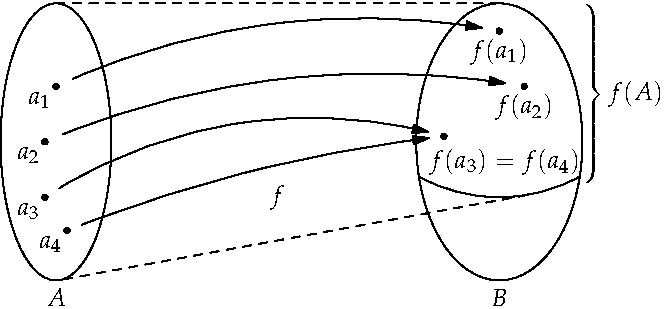
\includegraphics[width=0.6\textwidth]{sets-16-funcdef}
\end{center}



\begin{minipage}[t]{0.62\linewidth}\vspace{0pt}
		For simple real-valued functions, the domain and range are easily seen in a graph. For instance if $f:[-3,2)\to\R$ is the square function
		\[f:x\mapsto x^2,\]
		then we have $\dom(f)=[-3,2)$ and $\range(f)=[0,9]$, as seen in the picture. We could also calculate other images, for example,
  	\[f\bigl([-1,2)\bigr)=[0,4).\]
  \end{minipage}\hfill
  \begin{minipage}[t]{0.33\linewidth}\vspace{0pt}
  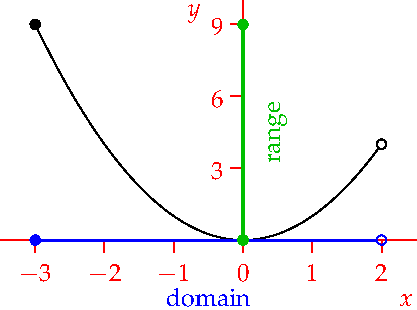
\includegraphics[scale=1]{sets-10-rangedom}
  \end{minipage}\par
  
 For most functions we will not be able to sketch a graph. Here are several examples where a graph is either unhelpful, or simply impossible to draw!
  
\begin{examples}{}{}
\begin{enumerate}
  \item Define $f:\Z\to\{0,1,2\}$ by $f:n\mapsto n^2\pmod 3$, where we take the remainder of $n^2$ modulo 3. Clearly $\dom(f)=\Z$, but what is the range? Trying a few examples, we see the following:
  \[\begin{array}{c|ccccccccccc}
  n&0&1&2&3&4&5&6&7&8&9&10\\\hline
  f(n)&0&1&1&0&1&1&0&1&1&0&1
  \end{array}\]
  It looks like the range is simply $\{0,1\}$. We have already proved this fact in Theorem ????!!!! EXERCISE ???, although a faster proof can now be given by appealing to modular arithmetic (Section \ref{sec:cong}).
  \begin{itemize}\setlength{\itemsep}{0pt}
    \item[] If $n\equiv 0$, then $n^2\equiv 0\pmod 3$.
    \item[] If $n\equiv 1$, then $n^2\equiv 1\pmod 3$.
    \item[] If $n\equiv 2$, then $n^2\equiv 4\equiv 1\pmod 3$.
  \end{itemize}
  Thus $n^2\equiv 0,1\pmod 3$, and $\range(f)=\{0,1\}$.
  \item\label{ex:functmod1} Let $A=\{0,1,2,\ldots,9\}$ be the set of remainders modulo 10 and define $f:A\to A$ by $f:n\mapsto 3n\pmod{10}$. To help understand this function, list the elements: the domain only has 10 elements after all.
  \[\begin{array}{c|cccccccccc}
  n&0&1&2&3&4&5&6&7&8&9\\\hline
  f(n)&0&3&6&9&2&5&8&1&4&7
  \end{array}\]
  It should be obvious that $\range(f)=A$.
  \item\label{ex:functmod2} With the same notation as the previous example, let $g:A\to A:n\mapsto 4n\pmod{10}$. Now we have the following table:
  \[\begin{array}{c|cccccccccc}
  n&0&1&2&3&4&5&6&7&8&9\\\hline
  g(n)&0&4&8&2&6&0&4&8&2&6
  \end{array}\]
  with $\range(g)=\{0,2,4,6,8\}$.
  \item Let $A=\{1,2,3,4,5\}$ and let $B=\{$two-element subsets of $A\}$. We define
  \[f:A\to B:a\mapsto\begin{cases}
  \{a,a+1\}&\text{if }a\neq 5,\\
  \{5,1\}&\text{if }a=5.
  \end{cases}\]
  This is tricky to read, since $B$ is a set of sets. You should be able to convince yourself that
  \[\range(f)=\big\{\{1,2\},\{2,3\},\{3,4\},\{4,5\},\{5,1\}\big\}\]
  and, for example, that
  \[f\big\{1,4\big\}=\big\{f(1),f(4)\big\}=\big\{\{1,2\},\{4,5\}\big\}\]
\end{enumerate}
\end{examples}


\boldsubsubsection{Injections, surjections and bijections}

\begin{defn}{}{11}
A function $f:A\to B$ is \emph{1--1} (one-to-one), \emph{injective}, or an \emph{injection} if it never takes the same value twice. Equivalently,\footnote{This is the contrapositive: if $f$ never takes the same value twice, then $\forall a_1, a_2\in A$ we have $a_1\neq a_2\implies f(a_1)\neq f(a_2)$.}
\[\forall a_1,a_2\in A,\ f(a_1)=f(a_2)\implies a_1=a_2.\]
$f:A\to B$ is \emph{onto}, \emph{surjective}, or a \emph{surjection} if it takes every value in the codomain: i.e., $B=\range(f)$. Equivalently,\footnote{This is the statement $B\subseteq\range(f)$. The opposite inclusion $\range(f)\subseteq B$ is true for \emph{any} function.}
\[\forall b\in B,\ \exists a\in A\text{ such that }f(a)=b.\]
$f:A\to B$ is \emph{invertible}, \emph{bijective}, or a \emph{bijection} if it is both injective and surjective.
\end{defn}

 Since the definitions of injective and surjective are both `for all' statements, to show that a function is \emph{not injective} or \emph{not surjective} you will need \emph{counterexamples.} For instance, consider the quadratic function $f:[-3,2)\to\R:x\mapsto x^2$ seen above. It is straightforward to see that $f$ is neither injective nor surjective. Indeed we have the following counterexamples:
		\begin{itemize}%\setlength\itemsep{0pt}
  	  \item $f(-1)=f(1)$. If $f$ were injective, the values at 1 and $-1$ would have to be different.
  	  \item $81\in\R$, yet there is no $x\in[-3,2)$ such that $f(x)=81$. Thus $f$ is not surjective.
		\end{itemize}
With a small change to either the domain or codomain, we can easily create an injective or a surjective function. For instance we can shrink the domain to obtain two injective functions:
\[g:[0,2)\to\R:x\mapsto x^2\quad\text{and}\quad h:[-3,0]\to\R:x\mapsto x^2\]
\begin{center}
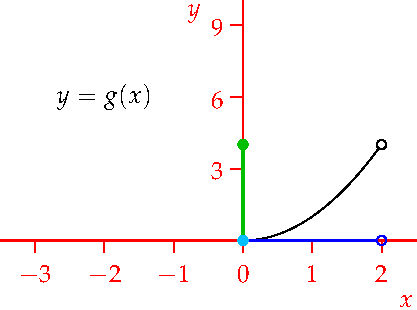
\includegraphics[width=0.4\textwidth]{sets-18-rangedom2}
\qquad\qquad\qquad
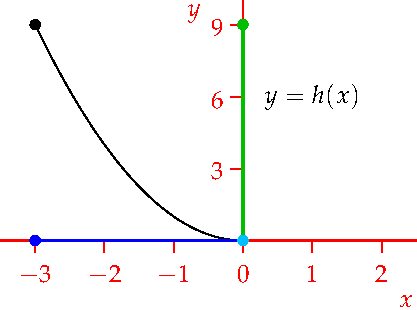
\includegraphics[width=0.4\textwidth]{sets-19-rangedom3}
\end{center}
To see this, note that
\[g(x_1)=g(x_2)\implies x_1^2=x_2^2\implies x_1=\pm x_2\implies x_1=x_2\]
since both must be non-negative. The argument for $h$ is similar.\\
By shrinking the codomain to equal the range we immediately create a surjective function:
\[j:[-3,2)\to [0,9]:x\mapsto x^2\]


Now consider the examples on page \pageref{ex:functmod1}. The details are provided for example 1. For the others, make sure you understand why the answer is correct. 
\begin{examples}{}{}
\begin{enumerate}
  \item $f:\Z\to\{0,1,2\}:n\mapsto n^2\pmod 3$ is neither injective nor surjective.
  	\begin{itemize}
  	  \item If $f$ were injective, then we could not have $f(1)=f(2)$.
  	  \item 2 is in the codomain $\{0,1,2\}$ of $f$, yet $2\notin\range(f)$, so $f$ is not surjective.
		\end{itemize}
  \item This is a bijection. Indeed $f$ is  a \emph{permutation,} a bijection from a set onto itself. To see injectivity, note that in the table
  \[\begin{array}{c|cccccccccc}
  n&0&1&2&3&4&5&6&7&8&9\\\hline
  f(n)&0&3&6&9&2&5&8&1&4&7
  \end{array}\]
  none of the values in the second row appears more than once. For surjectivity, observe that every element in the codomain $\{0,1,2,\ldots,9\}$ appears \emph{at least} once in the second row. Being bijective means that each element of the codomain appears \emph{exactly once.}
  \item Neither injective, nor surjective.
  \item Injective, but not surjective.
\end{enumerate}
\end{examples}


Here is a more complicated example.
\begin{example}{}{}
Prove that $f:\R\setminus\{1\}\to\R\setminus\{2\}$ defined by $f(x)=2+\frac 1{1-x}$ is bijective.\\[2pt]

\begin{minipage}{0.6\textwidth}
		\begin{itemize}
  	  \item[](Injectivity)\quad Suppose that $x_1$ and $x_2$ are in $\R\setminus\{1\}$, and $f(x_1)=f(x_2)$. Then
			\[2+\frac 1{1-x_1}=2+\frac 1{1-x_2}.\]
			A little elementary algebra shows that $x_1=x_2$, whence $f$ is injective.
  	  \item[](Surjectivity)\quad Let $y\in\R\setminus\{2\}$ and define $x=1-\frac 1{y-2}$. This makes sense since $y\neq 2$. Then
  	  \[f(x)=2+\frac 1{1-(1-\frac 1{y-2})}=y\]
  	  whence $f$ is surjective.
		\end{itemize}
  \end{minipage}\qquad
  \begin{minipage}{0.35\textwidth}
  	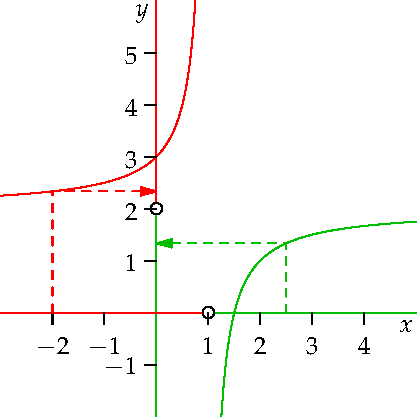
\includegraphics[width=\textwidth]{sets-09-bij}
  \end{minipage}\\[2pt]
The graphic is colored so that you can see how the different parts of the range and domain correspond. The argument for surjectivity is sneaky: how did we know to choose $x=1-\frac 1{y-2}$? The answer is scratch work: just solve $y=2+\frac 1{1-x}$ for $x$. Essentially we've shown that $f$ has the inverse function $f^{-1}(x)=1-\frac 1{x-2}$.
\end{example}

\begin{aside}{}{}
{\bf Inverse Functions}

The word \emph{invertible} is a synonym for bijective because bijective functions really have inverses! Indeed, suppose that $f:A\to B$ is bijective. Since $f$ is surjective, we know that $B=\range(f)$ and so every element of $B$ has the form $f(a)$ for some $a\in A$. Moreover, since $f$ is injective, the $a$ in question is unique. The upshot is that, when $f$ is bijective, we can construct a new \emph{function}
\[f^{-1}:B\to A:f(a)\mapsto a.\]
This may appear difficult at the moment but we will return to it in Chapter \ref{chap:relations}.

Instead, recall that in Calculus you saw that any injective function has an inverse. How does this fit with our definition? Consider, for example, $f:[0,2]\to\R:x\mapsto x^4$. This is injective but not surjective. To fix this, simply define a new function with the same formula but with codomain equal to the range of $f$. We obtain the bijective function
\[g:[0,2]\to[0,16]:x\mapsto x^4,\]
with inverse
\[g^{-1}:[0,16]\to[0,2]:x\mapsto \sqrt[4]{x}.\]
In Calculus we didn't nitpick like this and would simply go straight to $f^{-1}(x)=\sqrt[4]{x}$.\\[5pt]
In general, if $f:A\to B$ is any injective function, then $g:A\to f(A):x\mapsto f(x)$ is automatically bijective, since we are forcing the codomain of $g$ to match its range.
\end{aside}

\boldsubsubsection{Functions and Cardinality}

Injective and surjective functions are intimately tied to the notion of cardinality. Indeed, in Chapter \ref{chap:cantor}, we will use such functions to give a \emph{definition} of cardinality for infinite sets. For the present we stick to finite sets. 

\begin{thm}{}{finitecard}
Let $A$ and $B$ be finite sets. The following are equivalent:
\begin{enumerate}\setlength{\itemsep}{0pt}
  \item $\nm A\le\nm B$.
  \item $\exists f:A\to B$ injective.
  \item $\exists g:B\to A$ surjective.
\end{enumerate}
\end{thm}

\begin{minipage}{0.8\textwidth}
Read the theorem carefully. It is simply saying that, of the three statements, if \emph{any} one is true then \emph{all} are true. Similarly, if one is false then so are the others. It might appear that we require six arguments! Instead we illustrate an important technique: when showing that multiple statements are equivalent, it is enough to prove in a circle. For instance, if we prove the three implications indicated in the picture, then $\circint 1\Longrightarrow \circint 3$ will be true because \emph{both} $\circint 1\Longrightarrow \circint 2$ and $\circint 2\Longrightarrow \circint 3$ are true.\\
\end{minipage}\qquad
\begin{minipage}{0.15\textwidth}
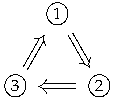
\includegraphics[width=\textwidth]{sets-14-circlearg}
\end{minipage}

 More generally, to show that $n$ statements are equivalent, only $n$ arguments are required.

 The proof may appear very abstract, but it is motivated by two straightforward pictures. Don't be afraid to use pictures to illustrate your proofs if it's going to make them easier to follow! If $\nm A=m$ and $\nm B=n$, then the two functions  can be displayed pictorially. Refer back to these pictures as you read through the proof.
\begin{center}
\begin{tabular}{c@{\hspace{1cm}}c}
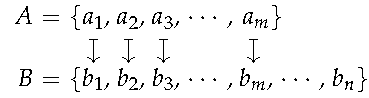
\includegraphics[scale=0.9]{sets-11-finiteinj}&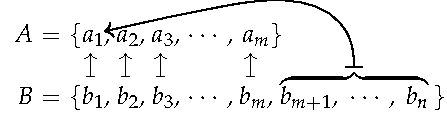
\includegraphics[scale=0.9]{sets-12-finiteinj}\\
The function $f$&The function $g$
\end{tabular}
\end{center}

\begin{proof}
The proof relies crucially on the fact that $A,B$ are finite. Suppose that $\nm A=m$ and $\nm B=n$ throughout and list the elements of $A$ and $B$ as,
\[A=\{a_1,a_2,\ldots,a_m\},\qquad\qquad B=\{b_1,b_2,\ldots,b_n\}.\]
\begin{tabular}{@{}p{0.13\textwidth}@{}p{0.87\textwidth}@{}}
$\bigl(\circint 1\Longrightarrow \circint 2\bigr)$&Assume that $m\le n$. Define $f:A\to B$ by $f(a_k)=b_k$. This is injective since the elements $b_1,\ldots,b_m$ are distinct.\\
$\bigl(\circint 2\Longrightarrow \circint 3\bigr)$&Suppose that $f:A\to B$ is injective. Without loss of generality we may assume that the elements of $A$ and $B$ are labeled such that $f(a_k)=b_k$. Now define $g:B\to A$ by
  \[g(b_k)=\begin{cases}
  a_k&\text{ if }k\le m,\\
  a_1&\text{ if }k>m.
  \end{cases}\]
  Then $g$ is surjective since every element $a_k$ is in the image of $g$.\\
$\bigl(\circint 3\Longrightarrow \circint 1\bigr)$&Finally suppose that $g:B\to A$ is surjective. Without loss of generality we may assume that $a_k=g(b_k)$ for $1\le k\le m$. Thus $n\ge m$.\qedhere  
\end{tabular}
\end{proof}

 It is worth noting in the proof of $\bigl(\circint 3\Longrightarrow \circint 1\bigr)$ that the elements $b_{m+1},\ldots,b_n$ may be mapped \emph{anywhere,} not just to $a_1$ as suggested in the picture above.

 If you read the proof carefully, it should be clear that when $m=n$, the function $f$ is actually a \emph{bijection} (with inverse $f^{-1}=g$).


\begin{cor}{}{finitecard}
If $A,B$ are finite sets, then $\nm A=\nm B\iff\exists f:A\to B$ bijective.
\end{cor}

\begin{proof}
Suppose that $m=n$. The argument $\circint 1\Longrightarrow \circint 2$ creates an injective function $f:A\to B$. However every element $b_k\in B$ is in the image of $f$, so this function is also surjective. Hence $f$ is a bijection.\\
Conversely, if $f:A\to B$ is a bijection, then it is injective, whence $m\le n$. It is also surjective, from which $n\le m$. Therefore $m=n$. 
\end{proof}


\boldsubsubsection{Composition of functions}

Finally, we consider composing function and, more particularly, how injectivity and surjectivity interact with composition.

\begin{defn}{}{}
Suppose that $f:A\to B$ and $g:B\to C$ are functions. The \emph{composition} $g\circ f:A\to C$ is the function defined by $(g\circ f)(a)=g(f(a))$.
\end{defn}
Note the order: to compute $(g\circ f)(x)$, you apply $f$ first, then $g$.

\begin{center}
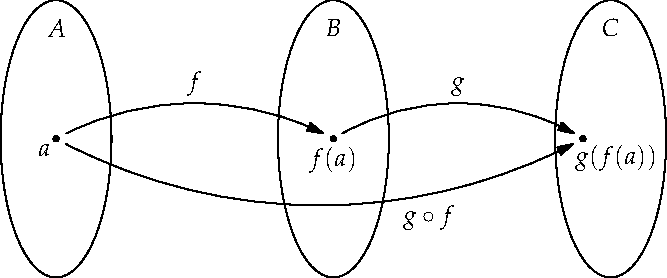
\includegraphics[width=0.65\textwidth]{sets-15-setcomp}
\end{center}

\begin{example}{}{}
If $f(x)=x^2$ and $g(x)=\frac 1{x-1}$, then
\[(g\circ f)(x)=\frac 1{x^2-1},\quad\text{and}\quad(f\circ g)(x)=\frac 1{(x-1)^2}.\]
You should be extra careful of ranges and domains when composing functions. The domain and range are not always explicitly mentioned, and at times some restriction of the domain is implied. In this example, you might assume that $\dom(f)=\R$ and $\dom(g)=\R\setminus\{1\}$. This is perfectly good if we are considering $f$ and $g$ separately. However, it should be clear from the formulæ that the implied domains of the compositions are,
\[\dom(g\circ f)=\R\setminus\{\pm 1\},\quad\text{and}\quad\dom(f\circ g)=\R\setminus\{1\}.\]
\end{example}

Our first two results on composing injective and surjective functions is easy to remember.

\begin{thm}{}{compinjsurj}
Let $f:A\to B$ and $g:B\to C$ be functions. Then:
\begin{enumerate}
  \item If $f$ and $g$ are injective, then $g\circ f$ is injective.
  \item If $f$ and $g$ are surjective, then $g\circ f$ is surjective.
\end{enumerate}
It follows that the composition of bijective functions is also bijective.
\end{thm}

\begin{proof}
\begin{enumerate}
  \item Suppose that $f$ and $g$ are injective and let $a_1,a_2\in A$ satisfy $(g\circ f)(a_1)=(g\circ f)(a_2)$. We are required to show that $a_1=a_2$. However,
  \begin{align*}
  (g\circ f)(a_1)=(g\circ f)(a_2)&\implies g\big(f(a_1)\big)=g\big(f(a_2)\big)\\
  &\implies f(a_1)=f(a_2)\tag*{(since $g$ is injective)}\\
  &\implies a_1=a_2\tag*{(since $f$ is injective)}\\[-25pt]
  \end{align*}\qedhere
%   \item Now suppose that $f$ and $g$ are surjective. Let $c\in C$. We are required to show that $\exists a\in A$ such that $(g\circ f)(a)=c$.\\
%   Since $g$ is surjective, $\exists b\in B$ such that $g(b)=c$.\\
%   Similarly, since $f$ is surjective, $\exists a\in A$ such that $f(a)=b$.\\
%   Together we have $(g\circ f)(a)=g(f(a))=c$, as required.
\end{enumerate}
\end{proof}

 Part 2 is in the Exercises. It is interesting to observe that the converse of this theorem is \emph{false.} Assuming that a composition is injective or surjective only forces \emph{one} of the original functions to be so.

\begin{thm}{}{}
Suppose that $f:A\to B$ and $g:B\to C$ are functions.
\begin{enumerate}
  \item If $g\circ f$ is injective, then $f$ is injective.
  \item If $g\circ f$ is surjective, then $g$ is surjective.
\end{enumerate}
\end{thm}

 Before showing the proof, consider the following representation of two functions $f$ and $g$ which simultaneously illustrate both parts of the theorem. It should be clear that $g\circ f$ is \emph{bijective,} $f$ is \emph{only injective,} and $g$ is \emph{only surjective.}

\begin{center}
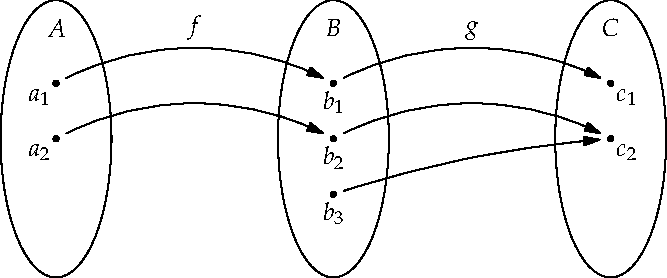
\includegraphics[width=0.65\textwidth]{sets-17-injcomp}
\end{center}

 Here is a formulaic example of the same thing. Make sure you're comfortable with the definitions and draw pictures or graphs to help make sense of what's going on.
\begin{gather*}
f:[0,2]\to[-4,4]:x\mapsto x^2\tag*{(injective only)}\\[5pt]
g:[-4,4]\to [0,16]:x\mapsto x^2\tag*{(surjective only)}\\[5pt]
g\circ f:[0,2]\to[0,16]:x\mapsto x^4\tag*{(bijective!)}
\end{gather*}


 This time we leave part 1 of the proof for the Exercises.
\begin{proof}
\begin{enumerate}\setcounter{enumi}{1}
%   \item Suppose that $f(a_1)=f(a_2)$. Then $(g\circ f)(a_1)=(g\circ f)(a_2)$. Since $g\circ f$ is injective we conclude that $a_1=a_2$, whence $f$ is injective.\qedhere
  \item Let $c\in C$ and assume that $g\circ f$ is surjective. We wish to prove that $\exists b\in B$ such that $g(b)=c$.\\
  Since $g\circ f$ is surjective, $\exists a\in A$ such that $(g\circ f)(a)=c$. But this says that
  \[g(f(a))=c.\]
  Hence $b=f(a)$ is an element of $B$ for which $g(b)=c$. Thus $g$ is surjective.\qedhere
\end{enumerate}
\end{proof}

% \paragraph{Self-test Questions}
% 
% 	\begin{enumerate}
%     \item $f:A\to B$ is \emph{injective} if \underline{\phantom{$f(a_1)=f(a_2)\implies a_1=a_2$\qquad\qquad}}
%     \item $f:A\to B$ is \emph{surjective} if \underline{\phantom{$\forall b\in B,\exists a\in A:f(a)=b$\qquad\qquad}}
%     \item If $f\circ g$ is bijective, which of the following \emph{must} be true?
%     \begin{itemize}
%       \item $f$ is injective.
%       \item $g$ is injective.
%       \item $f$ is surjective. 
%       \item $g$ is surjective.
%     \end{itemize}
%     \item True or false: We can always make a function surjective by making its domain smaller.
%     \item True or false: If $A$ is a subset of $B$ then there exists an injective function $f:A\to B$.
%   \end{enumerate}

\begin{exercises}

\begin{enumerate}
  \item For each of the following functions $f:A\to B$ determine whether $f$ is injective, surjective or bijective. Prove your assertions.
  \begin{enumerate}
    \item $f:[0,3]\to\R$ where $f(x)=2x$.
    \item $f:[3,12)\to[0,3)$ where $f(x)=\sqrt{x-3}$.
    \item $f:(-4,1]\to(-5,-3]$ where $f(x)=-\sqrt{x^2+9}$.
  \end{enumerate}
  
  \item Suppose that $f:[-3,\infty)\to[-8,\infty)$ and $g:\R\to\R$ are defined by
	\[f(x)=x^2+6x+1,\qquad\qquad g(x)=2x+3.\]
	Compute $g\circ f$ and show that $g\circ f$ is injective.
  
  \item Find:
		\begin{enumerate}
			\item A set $A$ so that the function $f:A\to\R:x\mapsto\sin x$ is injective.
			\item A set $B$ so that the function $f:\R\to B:x\mapsto\sin x$ is surjective.
		\end{enumerate}


  \item (\emph{If you did Exercise \ref*{sec:quant}.\ref{ex:decreasing} you should find this easy}) Let $X$ be a subset of $\R$. A function $f:X\to\R$ is \emph{strictly increasing} if 
	\[\forall \,a,\, b \in X,\quad a<b \Longrightarrow f(a)<f(b).\]
	For example, the function $f \colon [0,\,\infty)\to \R, \,x \mapsto x^2$  is increasing because 
	\[\forall a,\,b \in  [0,\,\infty) , \quad a<b \Longrightarrow f(a) = a^2< b^2=f(b).\]
		\begin{enumerate}
	  	\item Give another example of a function that is increasing. Draw its graph, and prove that  the function is increasing.  
	  	\item By negating the above definition, state what it means for a function \emph{not to be strictly increasing.} 
	  	\item Give an example of a function that is \emph{not} strictly increasing. Draw its graph, and prove that the function is not strictly increasing.  
	  	\item Let $f,\,g:\R\to\R$ be strictly increasing. Prove or disprove: The function $h=f+g$ is strictly increasing. Note that the formula for $h$ is $h(x)=f(x)+g(x)$.
		\end{enumerate}	
		
  \item You may assume that $g:[2,\infty)\to\R:x\mapsto \sqrt{x^3-8}$ is an injective function. Find a function $f:\R\to\R$ which is \emph{not injective,} but for which the composition $f\circ g:[2,\infty)\to\R$ \emph{is injective.} Justify your answer.

  \item A function $f:\R\to\R$ is \emph{even} if 
	\[\forall\,x\in\R,\ f(-x)=f(x).\]
	For example, the function $f:\R\to\R,\,x\mapsto x^2$ is even because 
	\[\forall\, x\in\R,\ f(-x)=(-x)^2= x^2=f(x).\]
	Note that $f$ is even if and only if the graph of $f$ is symmetric with respect to the $y$ axis. 
		\begin{enumerate}
	  	\item Give an example of a function that is even.  Draw its graph, and prove that  the function is even.
	  	\item Define what it means for a function \emph{not to be even}, by negating the definition above. 
	  	\item Give an example of a function that is \emph{not} even. Draw its graph, and prove that  the function is not even. 
	  	\item Prove or disprove: for every  $f ,\,g\colon \R \to \R$ even, the composition $ h= f\circ g$ is even. Here $h$ is the function mapping $x$ to $f(g(x))$.
		\end{enumerate}
	
  \item Define $f:(-\infty,0]\to\R$ and $g:[0,\infty)\to\R$ by
  \[f(x)=x^2,\qquad g(x)=\begin{cases}
  \frac{x}{1-x}&x<1,\\
  1-x&x\ge 1.
  \end{cases}\]
  Does $g\circ f$ map $(-\infty,0]$ onto $\R$? Justify your answer.
  
  \item Express, using quantifiers, what it means for a function to be
  \begin{enumerate}
    \item Not injective.
    \item Not surjective.
  \end{enumerate}
	
  \item Prove that the composition of two surjective functions is surjective.
  
  \item Suppose that $g\circ f$ is injective. Prove that $f$ is injective.
  
  \item In the proof of Theorem \ref{thm:finitecard} we twice invoked \emph{without loss of generality.} In both cases explain why the phrase applies.
  
  \item\label{ex:kfunc} Recall Examples \ref{ex:functmod1} and \ref{ex:functmod2} on page \pageref{ex:functmod1}.
  \begin{enumerate}
    \item Consider the nine functions $f_k:A\to A:x\mapsto kx\pmod{10}$, where $k=1,2,\ldots,9$. Find the range of $f_k$ for each $k$. Can you find a relationship between the cardinality of $\range(f_k)$ and $k$?
		\item More generally, let $A=\{0,1,2\ldots,n-1\}$ be the set of remainders modulo $n$. If $f_k:A\to A:x\mapsto kx\pmod n$, conjecture a relationship between $\nm{\range(f_k)}$, $k$ and $n$. You don't need to prove your assertions.
  \end{enumerate}
  
  
  ALE
  
    \item Let $f : \R \to \R^+$ be the function defined by $f(x) = e^x$. Explain why the following ``proof'' that $f$ is surjective is incorrect. Then, give a correct proof.  
\begin{proof}
Let $e^x \in \R^+$ be arbitrary. Then $f(x) = e^x$. So $f$ is surjective.
\end{proof}
	
  \item Prove that the composition of two surjective functions is surjective.
  
  \item Suppose that $g\circ f$ is injective. Prove that $f$ is injective.
  
  \item In the proof of Theorem \ref{thm:finitecard} we twice invoked \emph{without loss of generality.} In both cases explain why the phrase applies.
  
%  \item\label{ex:kfunc} Recall Examples \ref{ex:functmod1} and \ref{ex:functmod2} on page \pageref{ex:functmod1}.
%   \begin{enumerate}
%     \item Consider the nine functions $f_k:A\to A:x\mapsto kx\pmod{10}$, where $k=1,2,\ldots,9$. Find the range of $f_k$ for each $k$. Can you find a relationship between the cardinality of $\range(f_k)$ and $k$?
% 		\item More generally, let $A=\{0,1,2\ldots,n-1\}$ be the set of remainders modulo $n$. If $f_k:A\to A:x\mapsto kx\pmod n$, conjecture a relationship between $\nm{\range(f_k)}$, $k$ and $n$. You don't need to prove your assertions.
%   \end{enumerate}

\item Let $f : A \to B$ be a function. Let $X_1,X_2 \subseteq A$. Prove or disprove the following:
\begin{enumerate}
    \item $X_1 \subseteq X_2$ implies $f(X_1) \subseteq f(X_2)$.
    \item $f(X_1 \cup X_2) = f(X_1) \cup f(X_2)$.
    \item $f(X_1 \cap X_2) \subseteq f(X_1) \cap f(X_2)$. 
    \item $f(X_1) \cap f(X_2) \subseteq f(X_1 \cap X_2)$.
    %\item If $f$ is injective, then $f(X_1 \cap X_2) = f(X_1) \cap f(X_2)$.
    %\item $f(X_1) \setminus f(X_2) \subseteq f(X_1 \setminus X_2)$.
\end{enumerate}

\item Let $f : A \to B$ be a function. Suppose that $f(X_1 \cap X_2) = f(X_1) \cap f(X_2)$ for \textbf{all} $X_1,X_2 \subseteq A$. Show $f$ is injective.

\item \begin{enumerate}
    \item Let $A = \{a,b,c\}$ and $B = \{1,2,3,4\}$ and $f : A \to B$ be the function given by $f(a) = f(c) = 1$ and $f(b) = 3$. Compute $f^{-1}(\{1\})$, $f^{-1}(\{3\})$, $f^{-1}(\{1,3\})$, and $f^{-1}(\{2,4\})$. 
    \item Let $g : [-1,\infty) \to \R$ be $g(x) = x^2 + 2x + 1$. Compute $g^{-1}((0,2))$. 
    \item Let $h : \R \to \R$ be $h(x) = \sin x$. Find $h^{-1}(\{-1,1\})$. 
\end{enumerate}

\item Let $f : A \to B$ be a function and $Y_1,Y_2 \subseteq B$.
\begin{enumerate}
\item Prove $f^{-1}(Y_1 \cup Y_2) = f^{-1}(Y_1) \cup f^{-1}(Y_2)$.
\item Prove $f^{-1}(Y_1 \cap Y_2) = f^{-1}(Y_1) \cap f^{-1}(Y_2)$.
\end{enumerate}

\item Let $f : A \to B$ be a function and let $X \subseteq A$. Fill in the details in the following to give a proof of the following two facts:
\begin{enumerate}
    \item $X \subseteq f^{-1}(f(X))$.
    \item If $f$ is injective, $X = f^{-1}(f(X))$.
\end{enumerate}

\item Let $f : A \to B$ be a function and let $Y \subseteq B$. Prove the following two facts:
\begin{enumerate}
    \item $f(f^{-1}(Y)) \subseteq Y$.
    \item If $f$ is surjective, $f(f^{-1}(Y)) = Y$.
\end{enumerate}

\item Let $A,B,C$, and $D$ be sets and $f : A \to B$, $g : B \to C$, and $h : C \to D$ be functions. Show that for all $a \in A$, we have
\[
(f \circ (g \circ h))(a) = ((f \circ g) \circ h)(a).
\]

\item (Uses calculus) This exercise will give an example of how to use calculus to prove some properties of (certain) functions. Let $f : (-\pi/2,\pi/2) \to \R$ be defined by $f(x) = \tan x$. Recall that $f$ is differentiable, and hence continuous, on its domain.
\begin{enumerate}
    \item Compute $\lim_{x \to \frac{\pi}{2}^-} f(x)$ and $\lim_{x \to \frac{-\pi}{2}^+} f(x)$.
    \item Recall the Intermediate Value Theorem: if $g : [a,b] \to \R$ is a continuous function, then for any $y$ between $g(a)$ and $g(b)$, there is $x \in [a,b]$ such that $g(x) = y$. Use the Intermediate Value Theorem and the results of part 1 to prove $f$ is surjective.
    \item Why is a strictly increasing function (see Exercise 4.4.4) injective? 
    \item Compute $\frac{d}{dx}f(x)$ and use this to show $f$ is strictly increasing, and therefore injective by part 3.
\end{enumerate}

\item Show there is a bijection between $\Z$ and $2\Z$.

\item Let $S$ be the set of all circles in the plane which are centered at the origin. Find a bijection between $S$ and $\R^+$.

\item Let $A$ and $B$ be \textbf{finite} sets. If $A \subsetneq B$, is it possible for there to be a bijection between $A$ and $B$?
\end{enumerate}

\end{exercises}

\fi